\documentclass[conference]{IEEEtran}
\IEEEoverridecommandlockouts
\usepackage[utf8]{inputenc}
\usepackage[T1]{fontenc}
\usepackage[spanish,es-nodecimaldot]{babel}
\usepackage{amsmath,amssymb}
\usepackage{booktabs}
\usepackage{graphicx}
\usepackage{float}
\usepackage{fancyhdr}
\usepackage{url}
\usepackage[hidelinks]{hyperref}
\usepackage{microtype}
\usepackage{caption}
\usepackage{enumitem}

\graphicspath{{diagramas/}{graficos/}{gráficos/}{../resultados/gráficos/}{../resultados/diagramas/}}
\setlength{\columnsep}{0.24in}
\setlength{\headheight}{14pt}
\pagestyle{fancy}
\fancyhf{}
\fancyfoot[C]{\footnotesize Documento elaborado con inteligencia artificial (GitHub Copilot en modo agente) para el curso IIC103G.}
\fancyheadoffset{0pt}
\renewcommand{\headrulewidth}{0pt}
\renewcommand{\footrulewidth}{0pt}
\fancypagestyle{plain}{%
  \fancyhf{}
  \fancyfoot[C]{\footnotesize Documento elaborado con inteligencia artificial (GitHub Copilot en modo agente) para el curso IIC103G.}
  \renewcommand{\headrulewidth}{0pt}
  \renewcommand{\footrulewidth}{0pt}
}

\title{Análisis de congestión vehicular mediante CMTD no homogéneas}
\author{}

\begin{document}
\twocolumn[
\begin{@twocolumnfalse}
\maketitle
\begin{center}
\textbf{Resumen}
\end{center}
\noindent\textbf{\hspace{1em}Este trabajo evalúa una hipótesis operacional sobre intersecciones urbanas semaforizadas usando una Cadena de Markov en Tiempo Discreto (CMTD) no homogénea y un modelo de utilización de cola. Se procesaron 204000 observaciones considerando 20 variables. Los datos consideraban los 7 días de la semana con diferentes regímenes climáticos. Las transiciones de estados de congestión se estimaron para regímenes horarios, climáticos y de fin de semana. Las pruebas $\chi^2$ rechazaron la homogeneidad entre franjas, climas y tipo de día ($p<0.001$). El ajuste no lineal de espera sobre $\rho=\lambda/\mu_{\mathrm{ef}}$ alcanzó $R^2=0.4223$, frente a $0.4152$ del ajuste lineal. Una simulación discreta reproducible produjo esperas medias crecientes entre $\rho=0.2$ y $\rho=0.9$. Los resultados apoyan una lectura dependiente del régimen, pero no establecen causalidad ni sustituyen aforos de campo.}

\medskip
\noindent\textbf{Palabras clave:} congestión urbana, CMTD no homogénea, teoría de colas, semáforos, simulación discreta.
\end{@twocolumnfalse}
]

\section{Introducción y contexto operacional}
La congestión en intersecciones urbanas semaforizadas es uno de los principales cuellos de botella de la movilidad contemporánea, ya que incrementa los tiempos de viaje, genera colas persistentes entre ciclos y reduce la confiabilidad de la red vial. Contar con modelos que distingan entre la variación horaria habitual y los cambios de régimen asociados a eventos climáticos o días de la semana permite a los equipos de operación anticipar episodios de saturación y priorizar ajustes en la programación semafórica.

En este contexto, el estado operativo de una intersección se representa mediante el espacio discreto $X_t \in \{\mathrm{Low},\mathrm{Moderate},\mathrm{High},\mathrm{Severe}\}$, evaluado hora a hora en un mismo tramo camino--intersección. Dado que la demanda y el desempeño vial varían durante el día y bajo distintas condiciones meteorológicas, se plantea que la evolución de $X_t$ sigue una Cadena de Markov en Tiempo Discreto (CMTD) no homogénea cuya matriz de transición depende de la franja horaria y del clima, mientras que los tiempos de espera en cola crecen de forma no lineal cuando el flujo se aproxima a la capacidad efectiva de servicio ($\rho = \lambda/\mu_{\mathrm{ef}}$).

En este informe se evalúa dicha hipótesis sobre registros horarios de 100 intersecciones semaforizadas. A continuación se presenta el marco teórico, el procedimiento aplicado para estimar las matrices condicionadas y analizar el comportamiento de colas, y la discusión de los resultados junto con sus implicancias y límites operacionales.

\section{Marco teórico}
Consideremos el proceso estocástico $\{X_n\}_{n\geq 0}$ sobre el espacio finito de estados de congestión
$S=\{\mathrm{Low},\mathrm{Moderate},\mathrm{High},\mathrm{Severe}\}$, donde
$n\in\{0,1,2,\ldots\}$ identifica cada instante horario consecutivo de observación.
El proceso satisface la propiedad de Markov cuando la distribución del estado futuro depende
del pasado únicamente a través del estado presente \cite{perez2026cmtd}. Para $i,j\in S$,
la probabilidad de transición en un paso se define como
\begin{equation}
p_{ij}=P(X_{n+1}=j\mid X_n=i).
\end{equation}
La matriz de transición $P=(p_{ij})_{i,j\in S}$ organiza el estado actual $i$ por filas
y el estado siguiente $j$ por columnas. Como sus entradas son probabilidades condicionales,
$p_{ij}\geq 0$ y cada fila satisface $\sum_{j\in S}p_{ij}=1$ \cite{perez2026cmtd}.

La cadena es homogénea cuando $p_{ij}$ no depende de $n$. Si la dinámica cambia según
un período o una condición externa, se formula como una CMTD no homogénea con una matriz
$P^{(r)}$ para cada régimen operativo $r$, definido aquí por franja horaria, clima o tipo
de día \cite{perez2026cmtd}. Esta formulación es consistente con el uso de cadenas de
Markov para sistemas dinámicos aleatorios y modelos de almacenamiento y colas descrito
por Douc et al. \cite{douc2018markov}.

Para estimar cada matriz se emplean frecuencias relativas:
\begin{equation}
\widehat{P}_{ij}^{(r)}=
\frac{N_{ij}^{(r)}}{\sum_{k\in S}N_{ik}^{(r)}}.
\end{equation}
Aquí, $N_{ij}^{(r)}$ es el número de transiciones horarias observadas desde el estado
actual $i$ hacia el estado siguiente $j$ bajo el régimen $r$. El denominador
$\sum_{k\in S}N_{ik}^{(r)}$ es el total de salidas registradas desde $i$ hacia cualquier
estado $k\in S$ en ese régimen. La homogeneidad entre regímenes se contrasta mediante una
prueba $\chi^2$ aplicada a las frecuencias de transición.

La tasa de llegada observada $\lambda$, expresada en vehículos por hora, se obtiene
directamente de los registros de flujo vehicular. La capacidad efectiva de servicio es
\begin{equation}
\mu_{\mathrm{ef}} = 60 \cdot L \cdot v_{\max} \cdot \frac{g}{C},
\end{equation}
donde $L$ es el número de pistas, $v_{\max}$ es la velocidad límite y $g/C$ es la
fracción efectiva de luz verde, calculada como la duración de la fase verde dividida
por el ciclo semafórico. El grado de saturación es $\rho=\lambda/\mu_{\mathrm{ef}}$.
Para $\rho<0.98$ se ajusta
\begin{equation}
W(\rho)=a+b\frac{\rho^k}{1-\rho},
\end{equation}
donde $W(\rho)$ es el tiempo medio de espera y $a$, $b$ y $k$ son parámetros estimados.
La forma funcional representa operacionalmente la acumulación de colas residuales entre
ciclos semafóricos: al aproximarse $\rho$ a uno, la demora crece de forma convexa y
acelerada, en lugar de lineal. Esta parametrización pertenece al diseño de este estudio;
no se presenta como una ley derivada de la bibliografía sobre cadenas de Markov.

\section{Datos y metodología}
\subsection{Preparación y observaciones}
La base de datos se obtuvo de \href{https://www.kaggle.com/datasets/mobeenfatimah/cityflow-smart-urban-mobility-and-traffic-iot}{CityFlow: Smart Urban Mobility and Traffic IoT (Kaggle)}. Corresponde a datos generados mediante una simulación de movilidad urbana e IoT, no a mediciones físicas directas en terreno. La copia de trabajo contenía 204000 filas y 47 columnas. El script \texttt{01\_preparar\_datos.py} conservó 20 variables: identificadores, fecha-hora, estados, variables de flujo, cola, señal y clima. El resultado contiene 204000 filas, 20 columnas y cero nulos; agrupa 100 pares \texttt{(road\_id,intersection\_id)}. La Figura~\ref{fig:pipeline} resume el flujo y la Figura~\ref{fig:arquitectura} conecta variables exógenas con ambos modelos.

\begin{figure}[H]
\centering
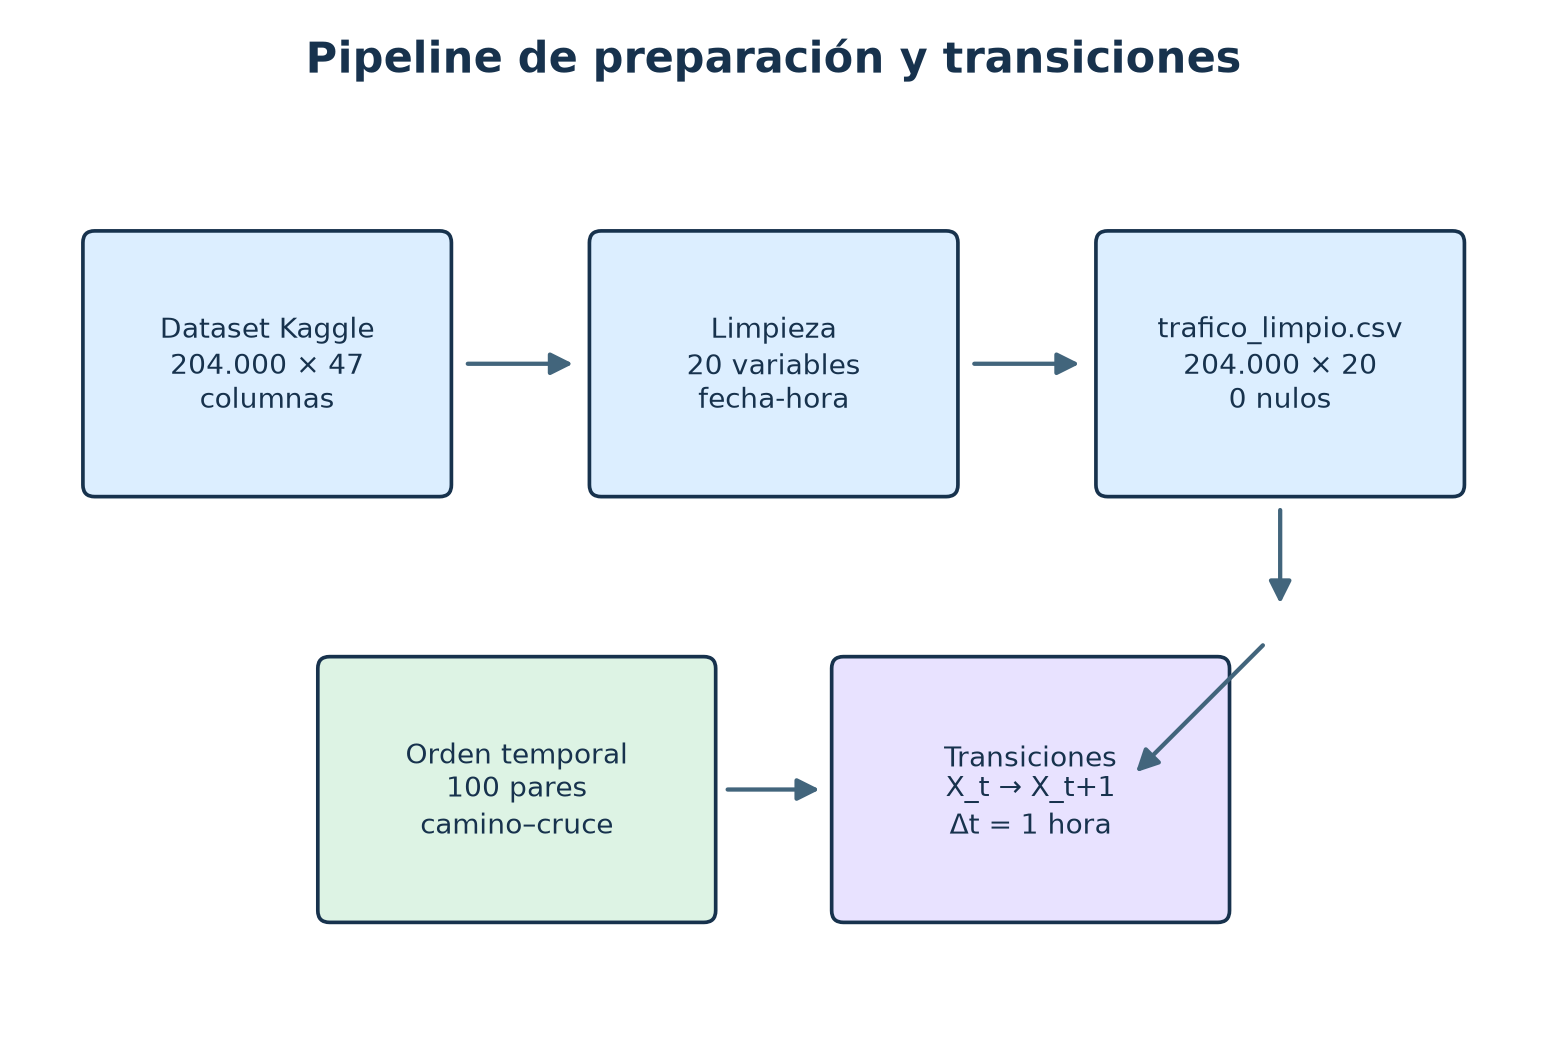
\includegraphics[width=\columnwidth]{diagrama_1_pipeline_datos.png}
\caption{Flujo reproducible de limpieza, ordenamiento y construcción de pares continuos.}
\label{fig:pipeline}
\end{figure}

\begin{figure}[H]
\centering
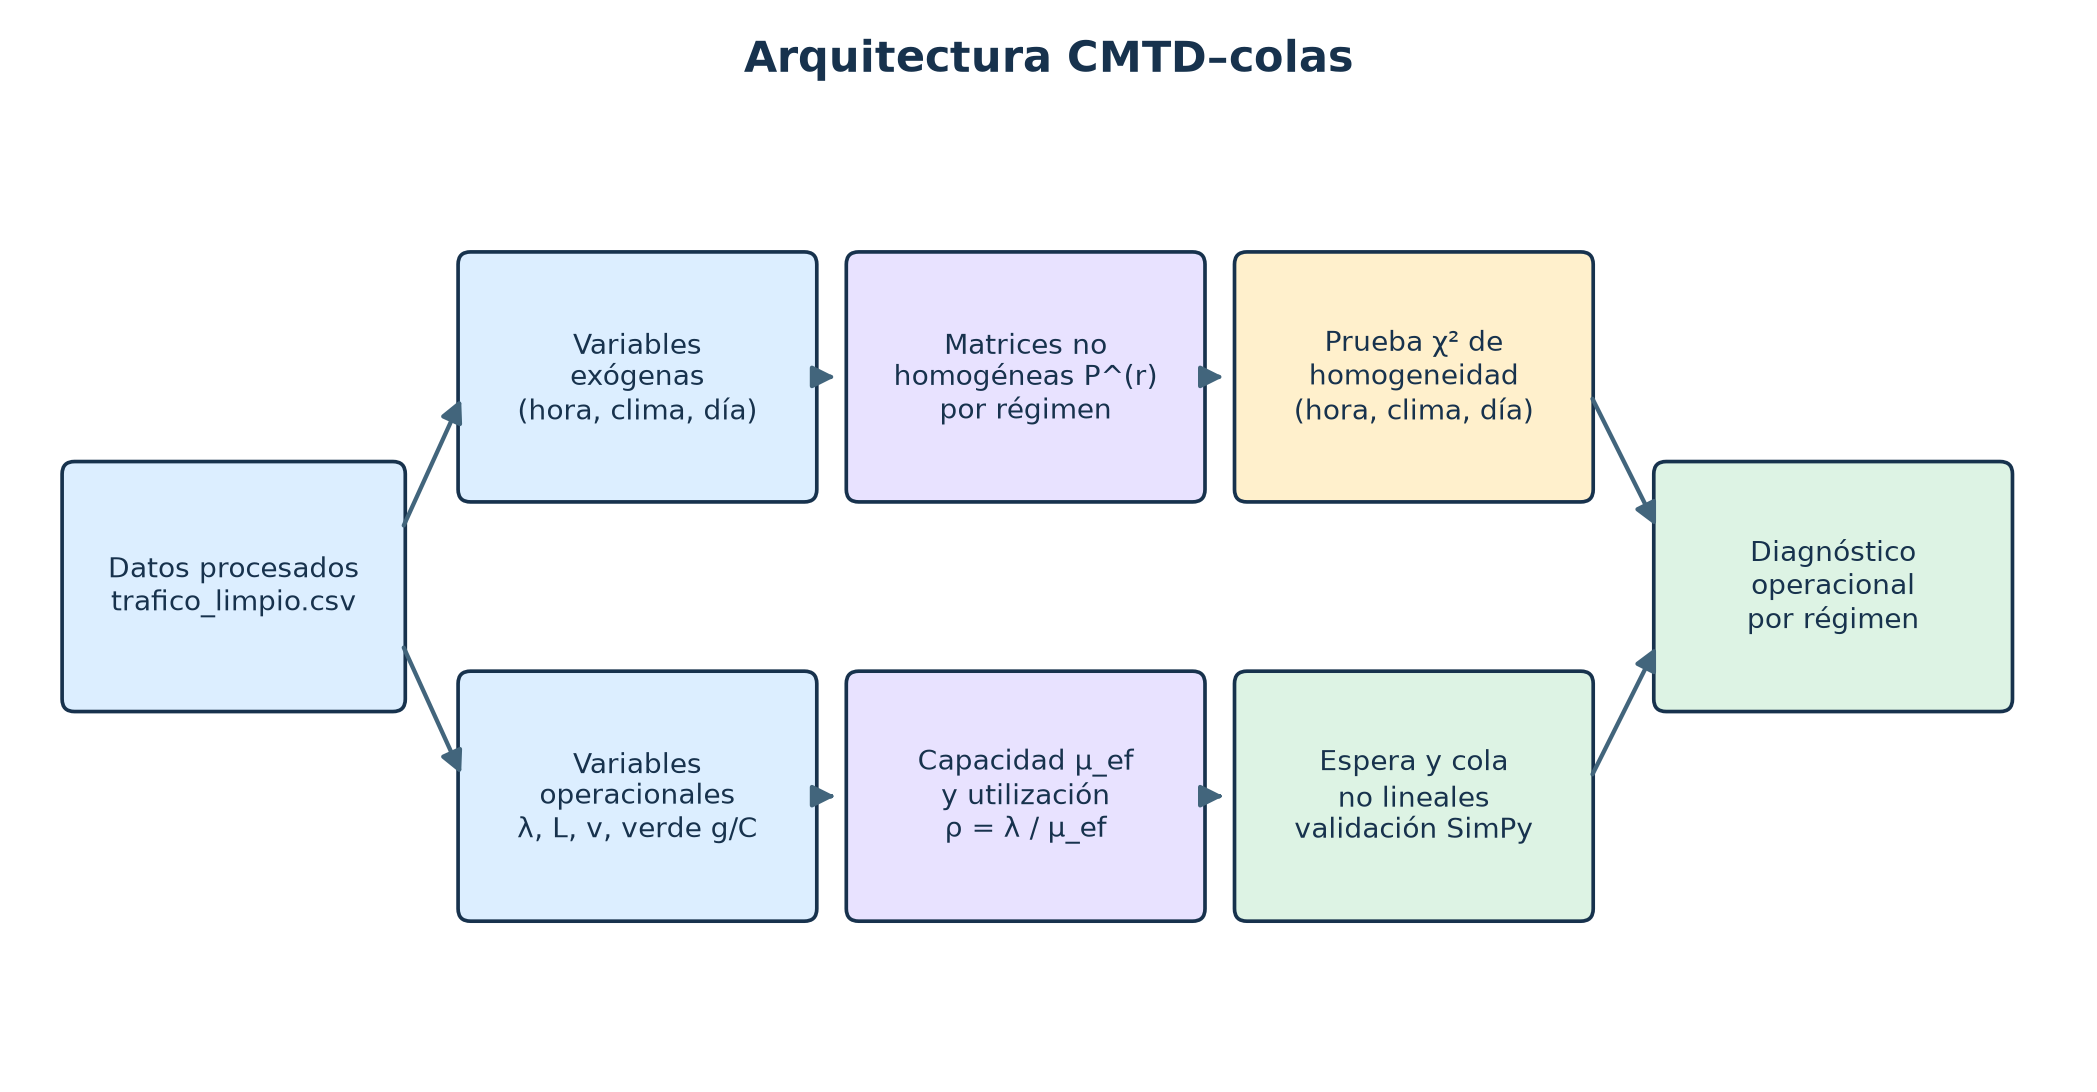
\includegraphics[width=\columnwidth]{diagrama_2_arquitectura_modelo.png}
\caption{Arquitectura conceptual CMTD--colas.}
\label{fig:arquitectura}
\end{figure}

Dentro de cada par camino--intersección se ordenaron las observaciones por marca temporal y se retuvieron únicamente las transiciones consecutivas separadas por una hora. Las matrices se estimaron para todos los cortes horarios, climáticos y semanales con el fin de ejecutar las pruebas globales $\chi^2$ de homogeneidad. Mientras tanto, el análisis comparativo detallado se concentra en los dos regímenes extremos: noche despejada (\texttt{Night | Clear}) y punta vespertina con lluvia (\texttt{Evening Peak | Rain}), como se visualiza directamente en las Figuras~\ref{fig:nightgraph} y~\ref{fig:raingraph}. La Figura~\ref{fig:trazabilidad} documenta la trazabilidad entre scripts, tablas, auditoría y entrega.

\begin{figure}[H]
\centering
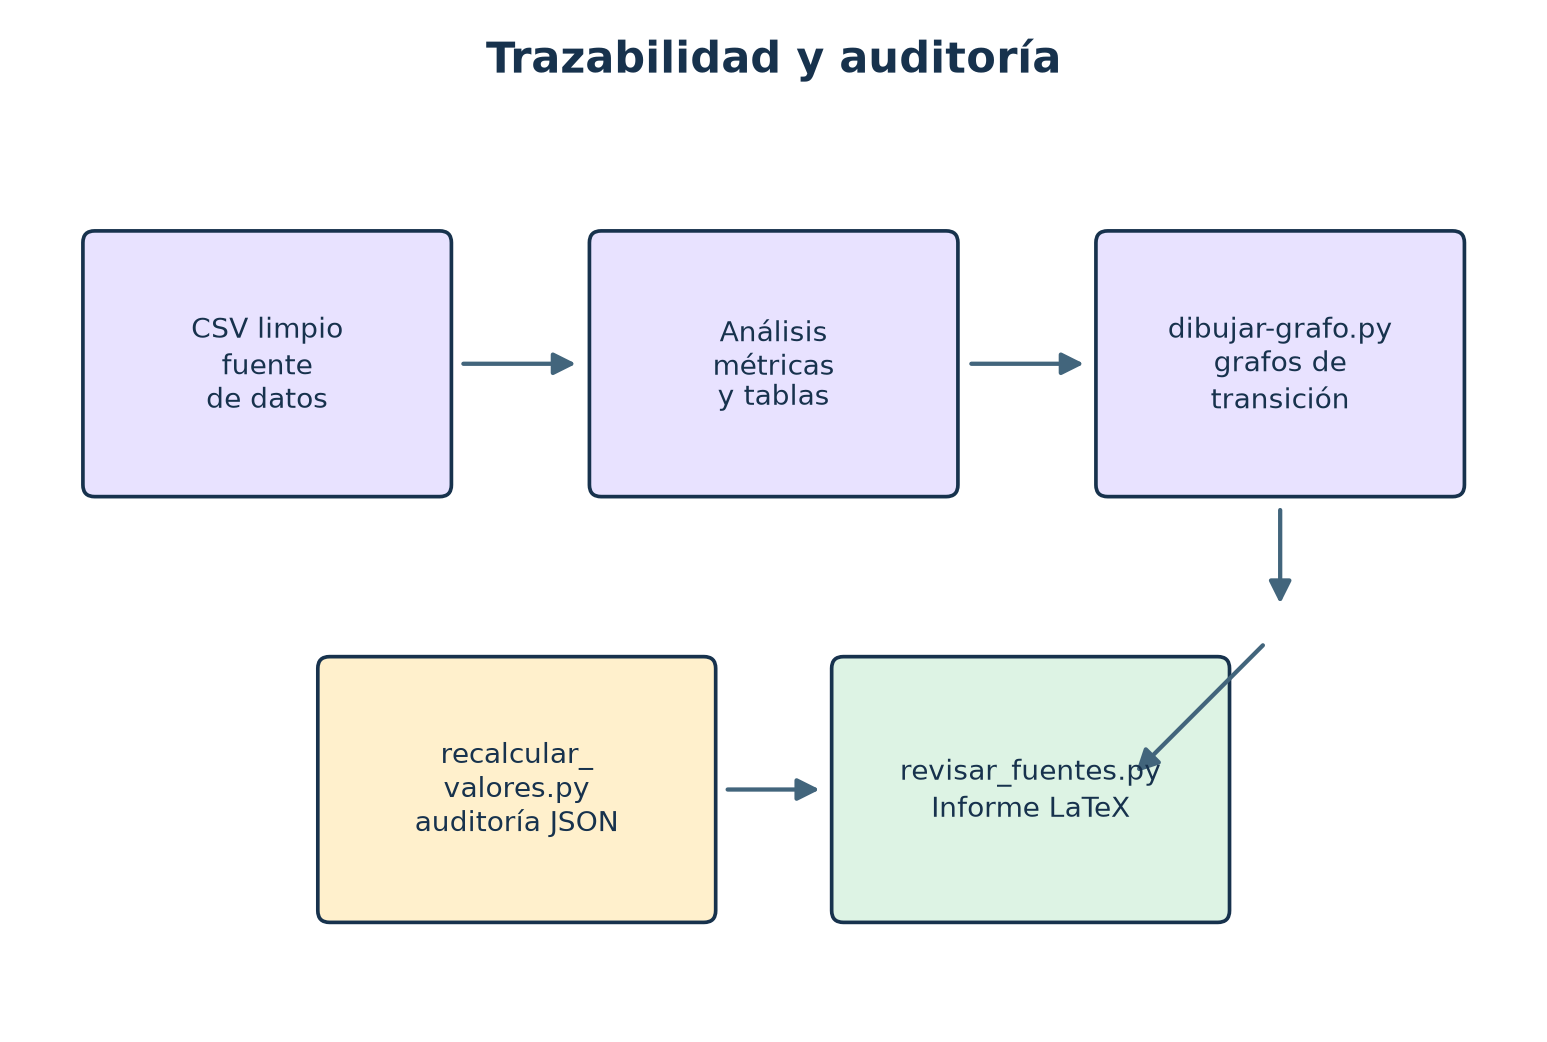
\includegraphics[width=\columnwidth]{diagrama_3_trazabilidad_auditoria.png}
\caption{Trazabilidad desde el CSV limpio hasta el informe.}
\label{fig:trazabilidad}
\end{figure}

\subsection{Simulación}
Dado que los registros del dataset presentan ruido operacional que dificulta aislar la
curvatura pura de la demora, se construyó una simulación de eventos discretos en SimPy
para verificar de forma controlada si el tiempo de espera crece no linealmente al acercarse
a la saturación ($\rho\rightarrow 1$).

La simulación modela una intersección semaforizada idealizada como un servidor FIFO con
llegadas aleatorias, ciclo de 2 minutos con 1 minuto de verde efectivo y servicio base de
0,5 minutos. La utilización se varió sistemáticamente en
$\rho\in\{0.2,0.4,0.6,0.8,0.9\}$ mediante tres réplicas con semillas fijas, horizonte de
1800 minutos y calentamiento de 300 minutos. La simulación valida cualitativamente la
dirección del crecimiento y no calibra una intersección física.

\section{Resultados y análisis}
\subsection{Dinámica Markoviana}
El contraste se concentra en \texttt{Night | Clear} y \texttt{Evening Peak | Rain} porque representan los dos extremos operacionales de la hipótesis: demanda mínima bajo clima favorable frente a alta demanda vespertina bajo lluvia. Esta selección permite visualizar el desplazamiento de la masa de transición sin saturar el informe con matrices intermedias, mientras las pruebas $\chi^2$ evalúan la no homogeneidad sobre todos los regímenes del conjunto de datos. En \texttt{Night | Clear}, $P(\mathrm{Low}\to\mathrm{Moderate})=0.0235$ y $P(\mathrm{Low}\to\mathrm{Low})=0.9764$. En \texttt{Evening Peak | Rain}, las probabilidades correspondientes son 0.0405 y 0.9595; además, $\mathrm{High}\to\mathrm{Moderate}=0.6163$ y $\mathrm{Severe}\to\mathrm{Severe}=0.1276$. Los grafos de ambos regímenes se muestran en las Figuras~\ref{fig:nightgraph} y~\ref{fig:raingraph}, y el mapa de calor de la Figura~\ref{fig:heatmap} permite comparar esas probabilidades visualmente.

\begin{figure}[H]
\centering
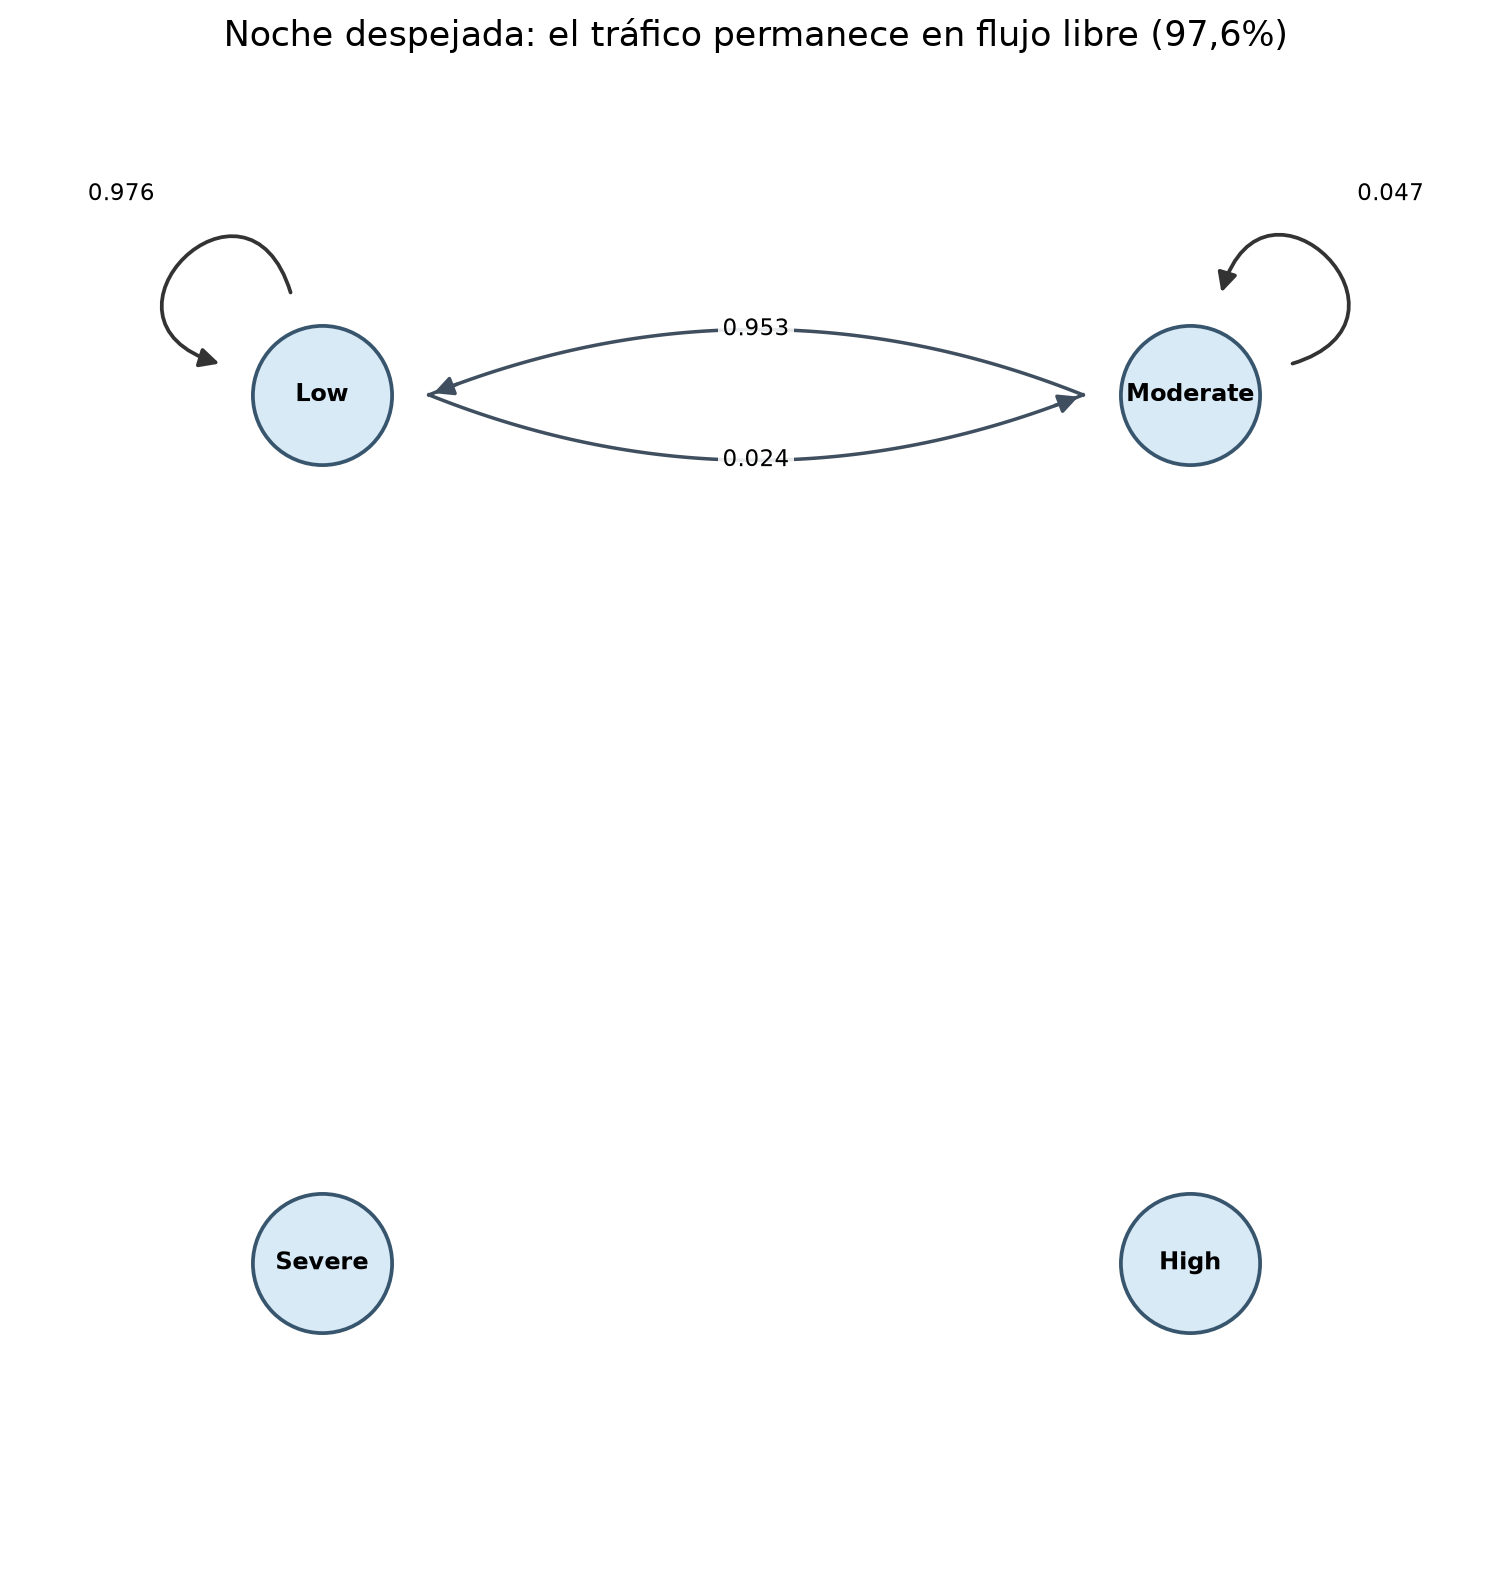
\includegraphics[width=.94\columnwidth]{grafo_night_clear.png}
\caption{Grafo de transición para Night | Clear.}
\label{fig:nightgraph}
\end{figure}

\begin{figure}[H]
\centering
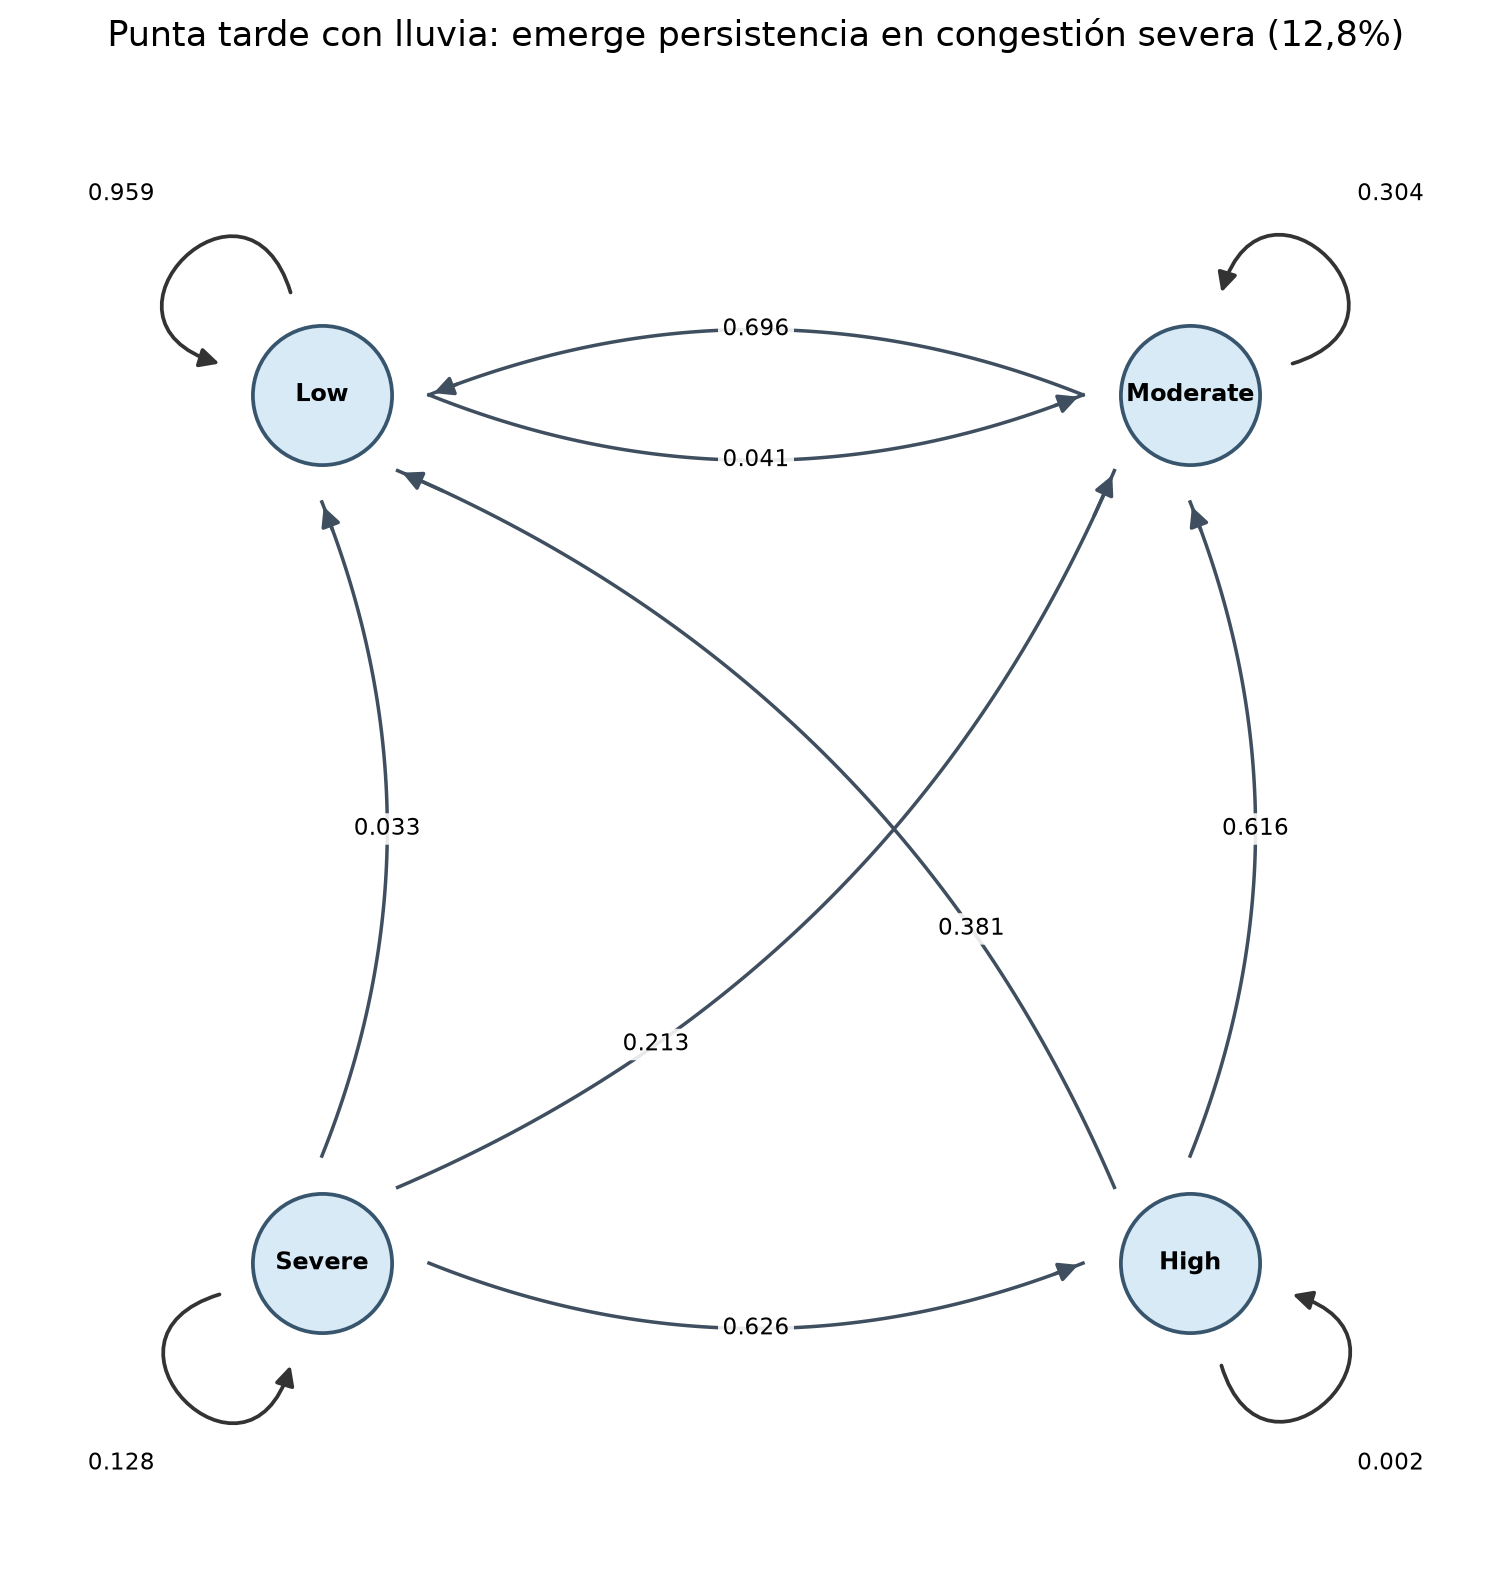
\includegraphics[width=.94\columnwidth]{grafo_evening_peak_rain.png}
\caption{Grafo de transición para Evening Peak | Rain.}
\label{fig:raingraph}
\end{figure}

La Figura~\ref{fig:heatmap} permite comparar visualmente las matrices y la Figura~\ref{fig:hourly} muestra la distribución empírica por hora, día laboral y fin de semana. La Tabla~\ref{tab:tests} resume los contrastes: horario ($\chi^2=308589.19$, 60 grados de libertad), clima ($\chi^2=5773.07$, 45) y tipo de día ($\chi^2=13834.22$, 15); todos presentan $p<0.001$. Por tanto, el supuesto de una única matriz común es incompatible con estas frecuencias observadas.
Sin embargo, con 204000 registros el tamaño muestral hace que diferencias pequeñas alcancen significación estadística; los resultados deben interpretarse junto con el tamaño de las celdas y el contraste visual entre matrices, no como magnitud uniforme del efecto.

\begin{figure}[H]
\centering
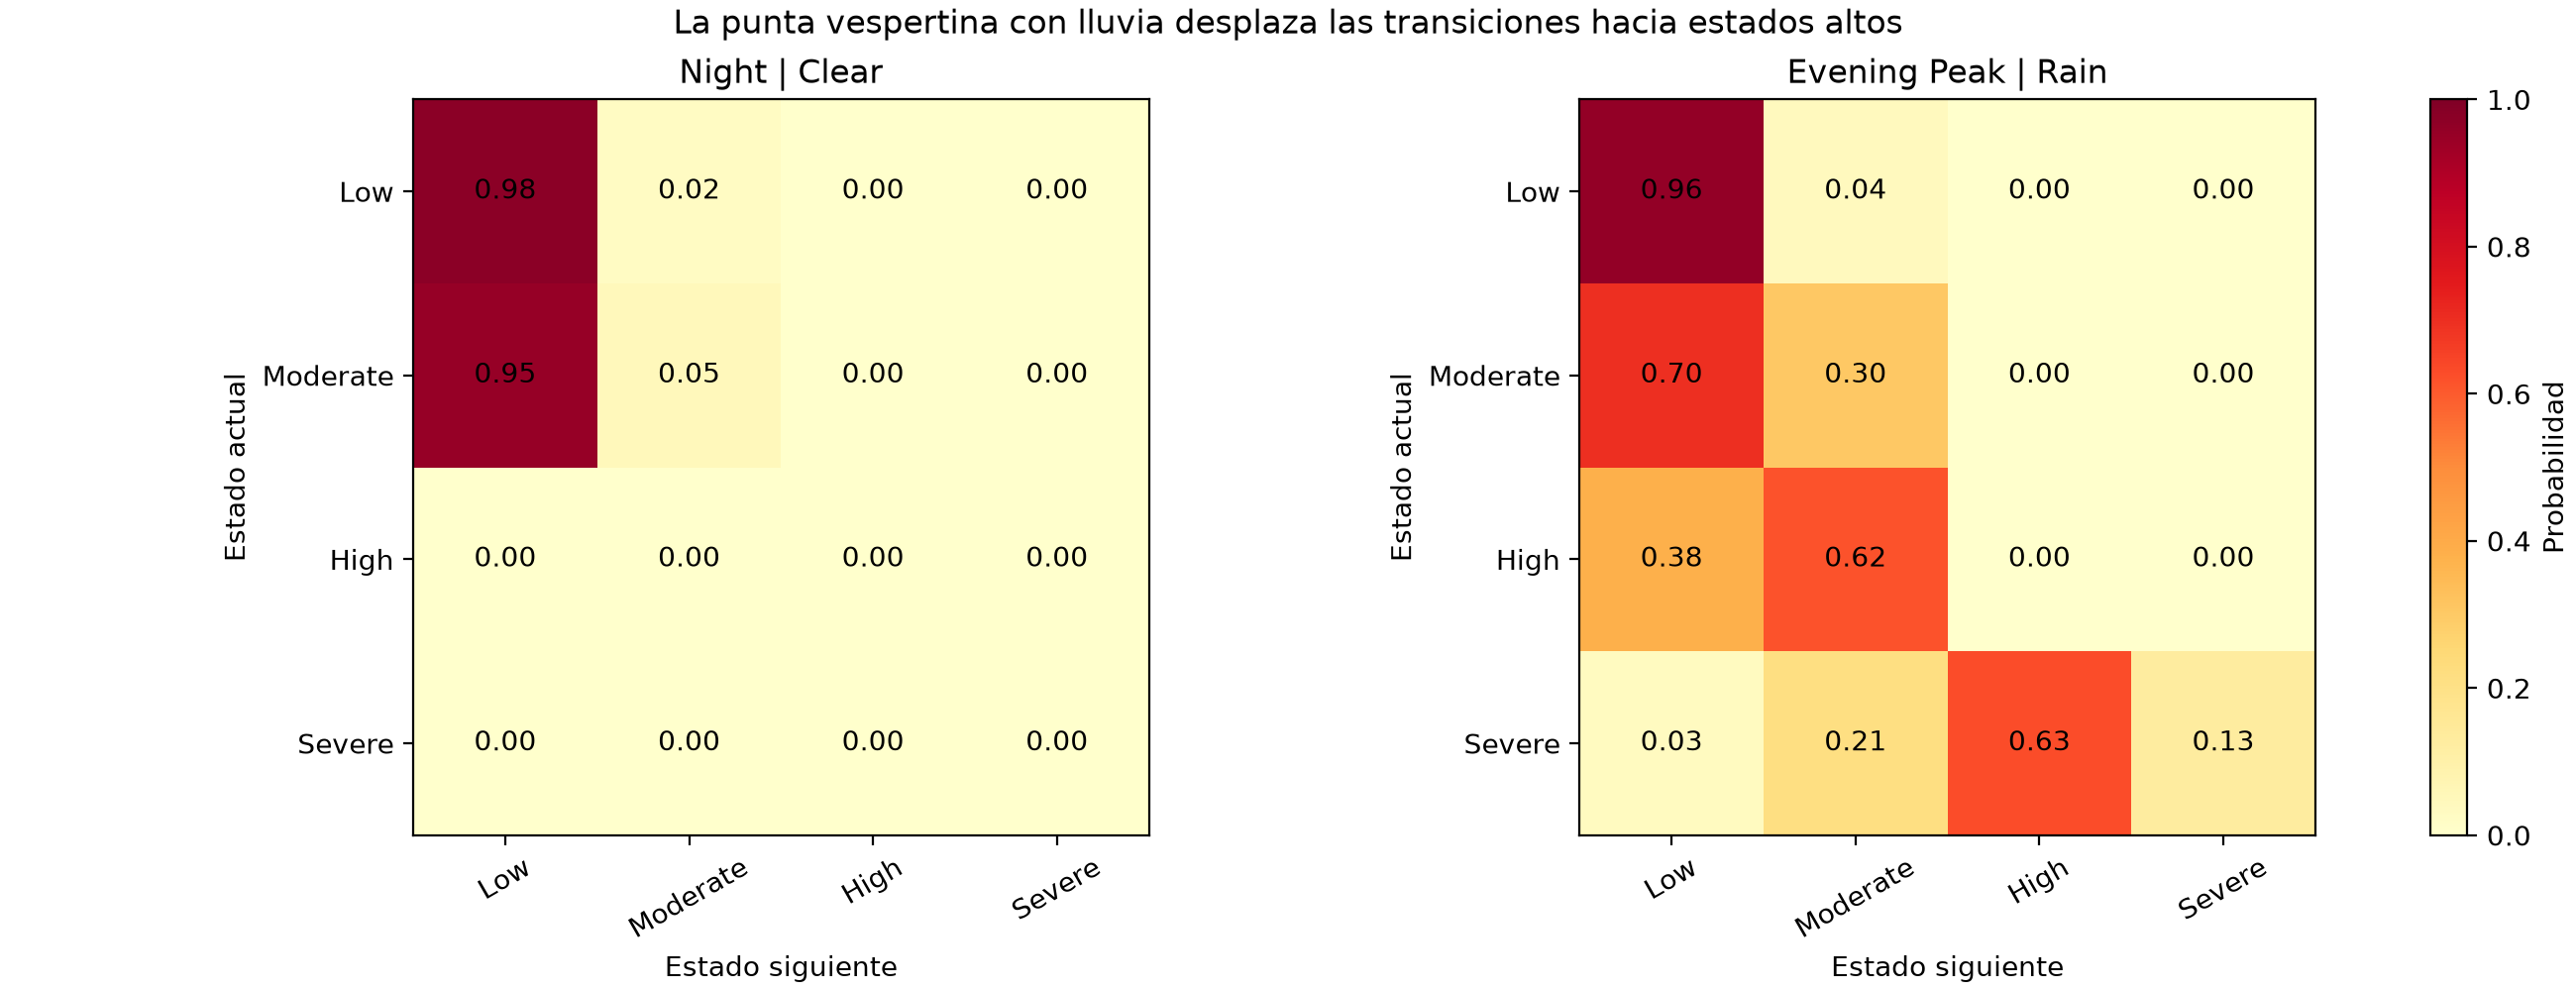
\includegraphics[width=\columnwidth]{heatmap_transiciones.png}
\caption{Comparación de matrices de transición en dos regímenes.}
\label{fig:heatmap}
\end{figure}

\begin{figure}[H]
\centering
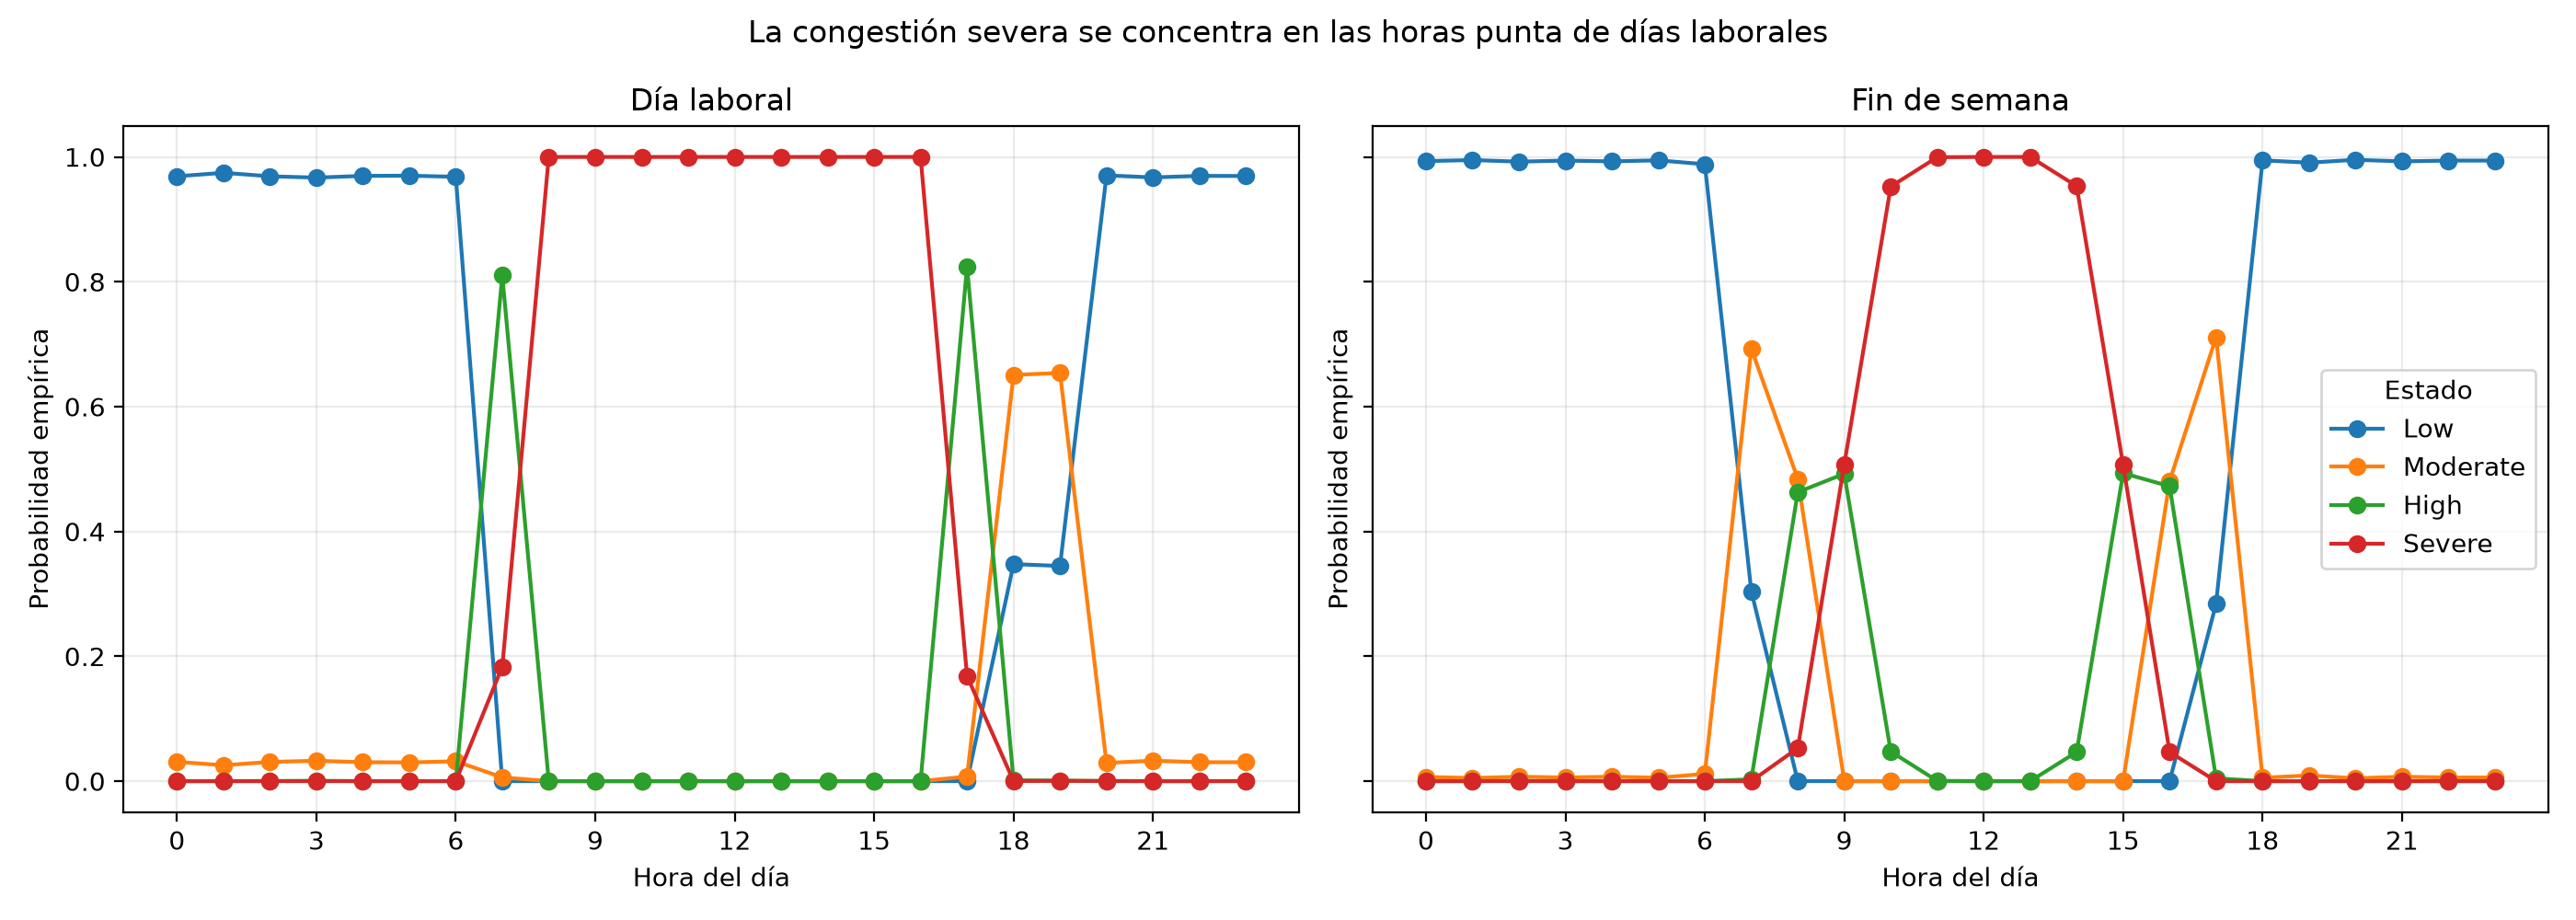
\includegraphics[width=\columnwidth]{evolucion_horaria_estados.png}
\caption{Probabilidad empírica de cada estado por hora y tipo de día.}
\label{fig:hourly}
\end{figure}

\begin{table}[H]
\caption{Pruebas $\chi^2$ de homogeneidad de frecuencias de transición.}
\label{tab:tests}
\centering\scriptsize
\begin{tabular}{lrrr}
\toprule
Variable & $\chi^2$ & gl & $p$\\
\midrule
Franja horaria&308589.19&60&$<.001$\\
Condición climática&5773.07&45&$<.001$\\
Tipo de día&13834.22&15&$<.001$\\
\bottomrule
\end{tabular}
\end{table}

\subsection{Saturación y colas}
Cada una de las 204000 observaciones horarias por intersección define un par $(\rho_i,W_i)$, donde $\rho_i=\lambda_i/\mu_{\mathrm{ef},i}$ es la utilización calculada y $W_i$ es el tiempo medio de espera observado en minutos. Sobre esta nube completa de puntos se ajustan por mínimos cuadrados tanto el modelo lineal $W(\rho)=a+b\rho$ ($R^2=0.4152$) como el modelo no lineal $W(\rho)=a+b\rho^k/(1-\rho)$ ($R^2=0.4223$). Dado que la alta densidad de puntos dificulta distinguir visualmente la curvatura, los registros se ordenan según $\rho$ y se agrupan en diez deciles de igual tamaño para graficar el promedio de espera de cada decil sobre ambas curvas ajustadas.

La Tabla~\ref{tab:queue} resume los deciles de $\rho$ y los parámetros del ajuste. La mejora no lineal es pequeña, por lo que la evidencia apoya una relación curvada, pero no demuestra una ventaja predictiva amplia. La Figura~\ref{fig:rho} muestra observaciones, medias por decil y ambos ajustes; la Figura~\ref{fig:box} desagrega espera y cola por estado y clima.

\begin{table}[H]
\caption{Resumen del ajuste de espera respecto de $\rho$.}
\label{tab:queue}
\centering\scriptsize
\begin{tabular}{lrr}
\toprule
Métrica & Lineal & No lineal\\
\midrule
$R^2$&.4152&.4223\\
Intercepto $a$&-7.6223&-5.0931\\
Pendiente $b$&131.9592&69.2316\\
Exponente $k$&--&.8664\\
Observaciones&204000&204000\\
\bottomrule
\end{tabular}
\end{table}

\begin{figure}[H]
\centering
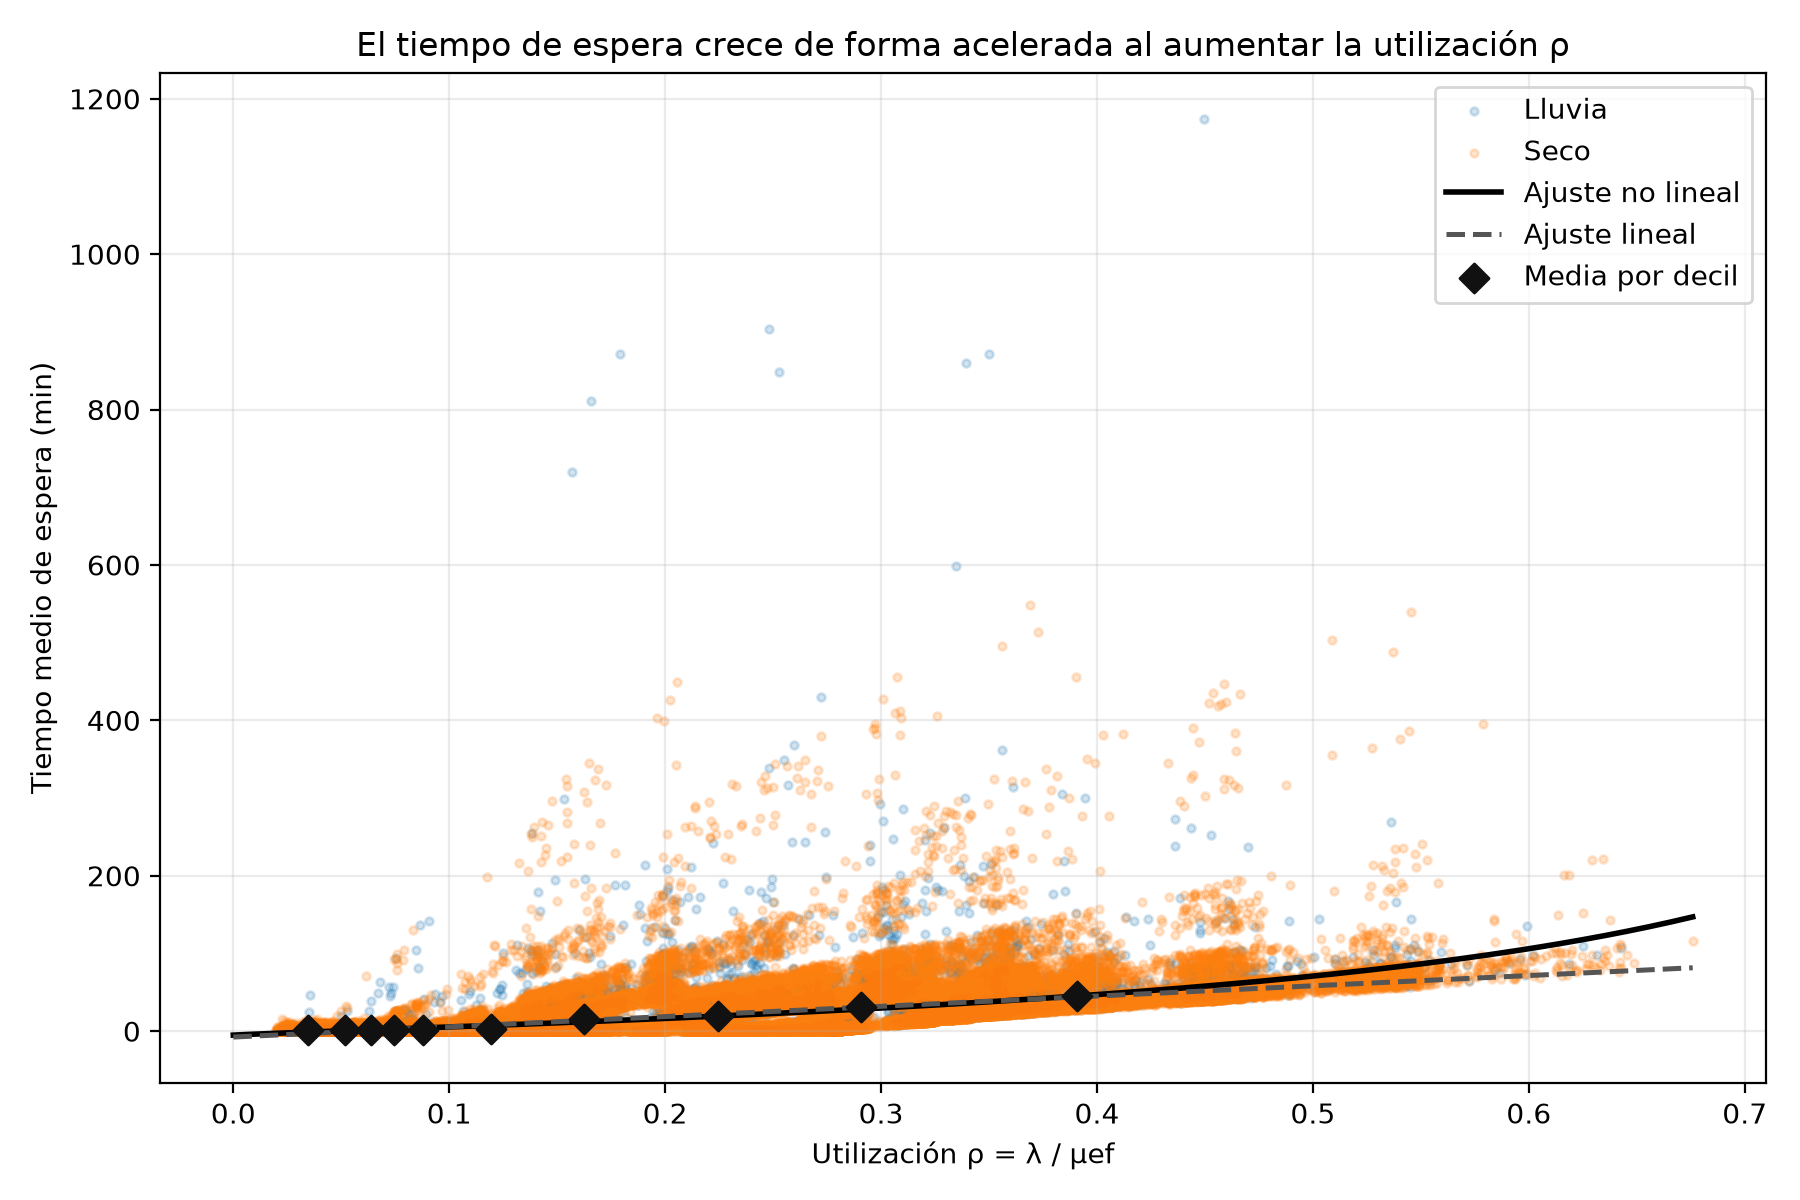
\includegraphics[width=\columnwidth]{espera_vs_utilizacion_rho.png}
\caption{Espera media frente a utilización, con ajuste lineal, ajuste no lineal y medias por decil.}
\label{fig:rho}
\end{figure}

\begin{figure}[H]
\centering
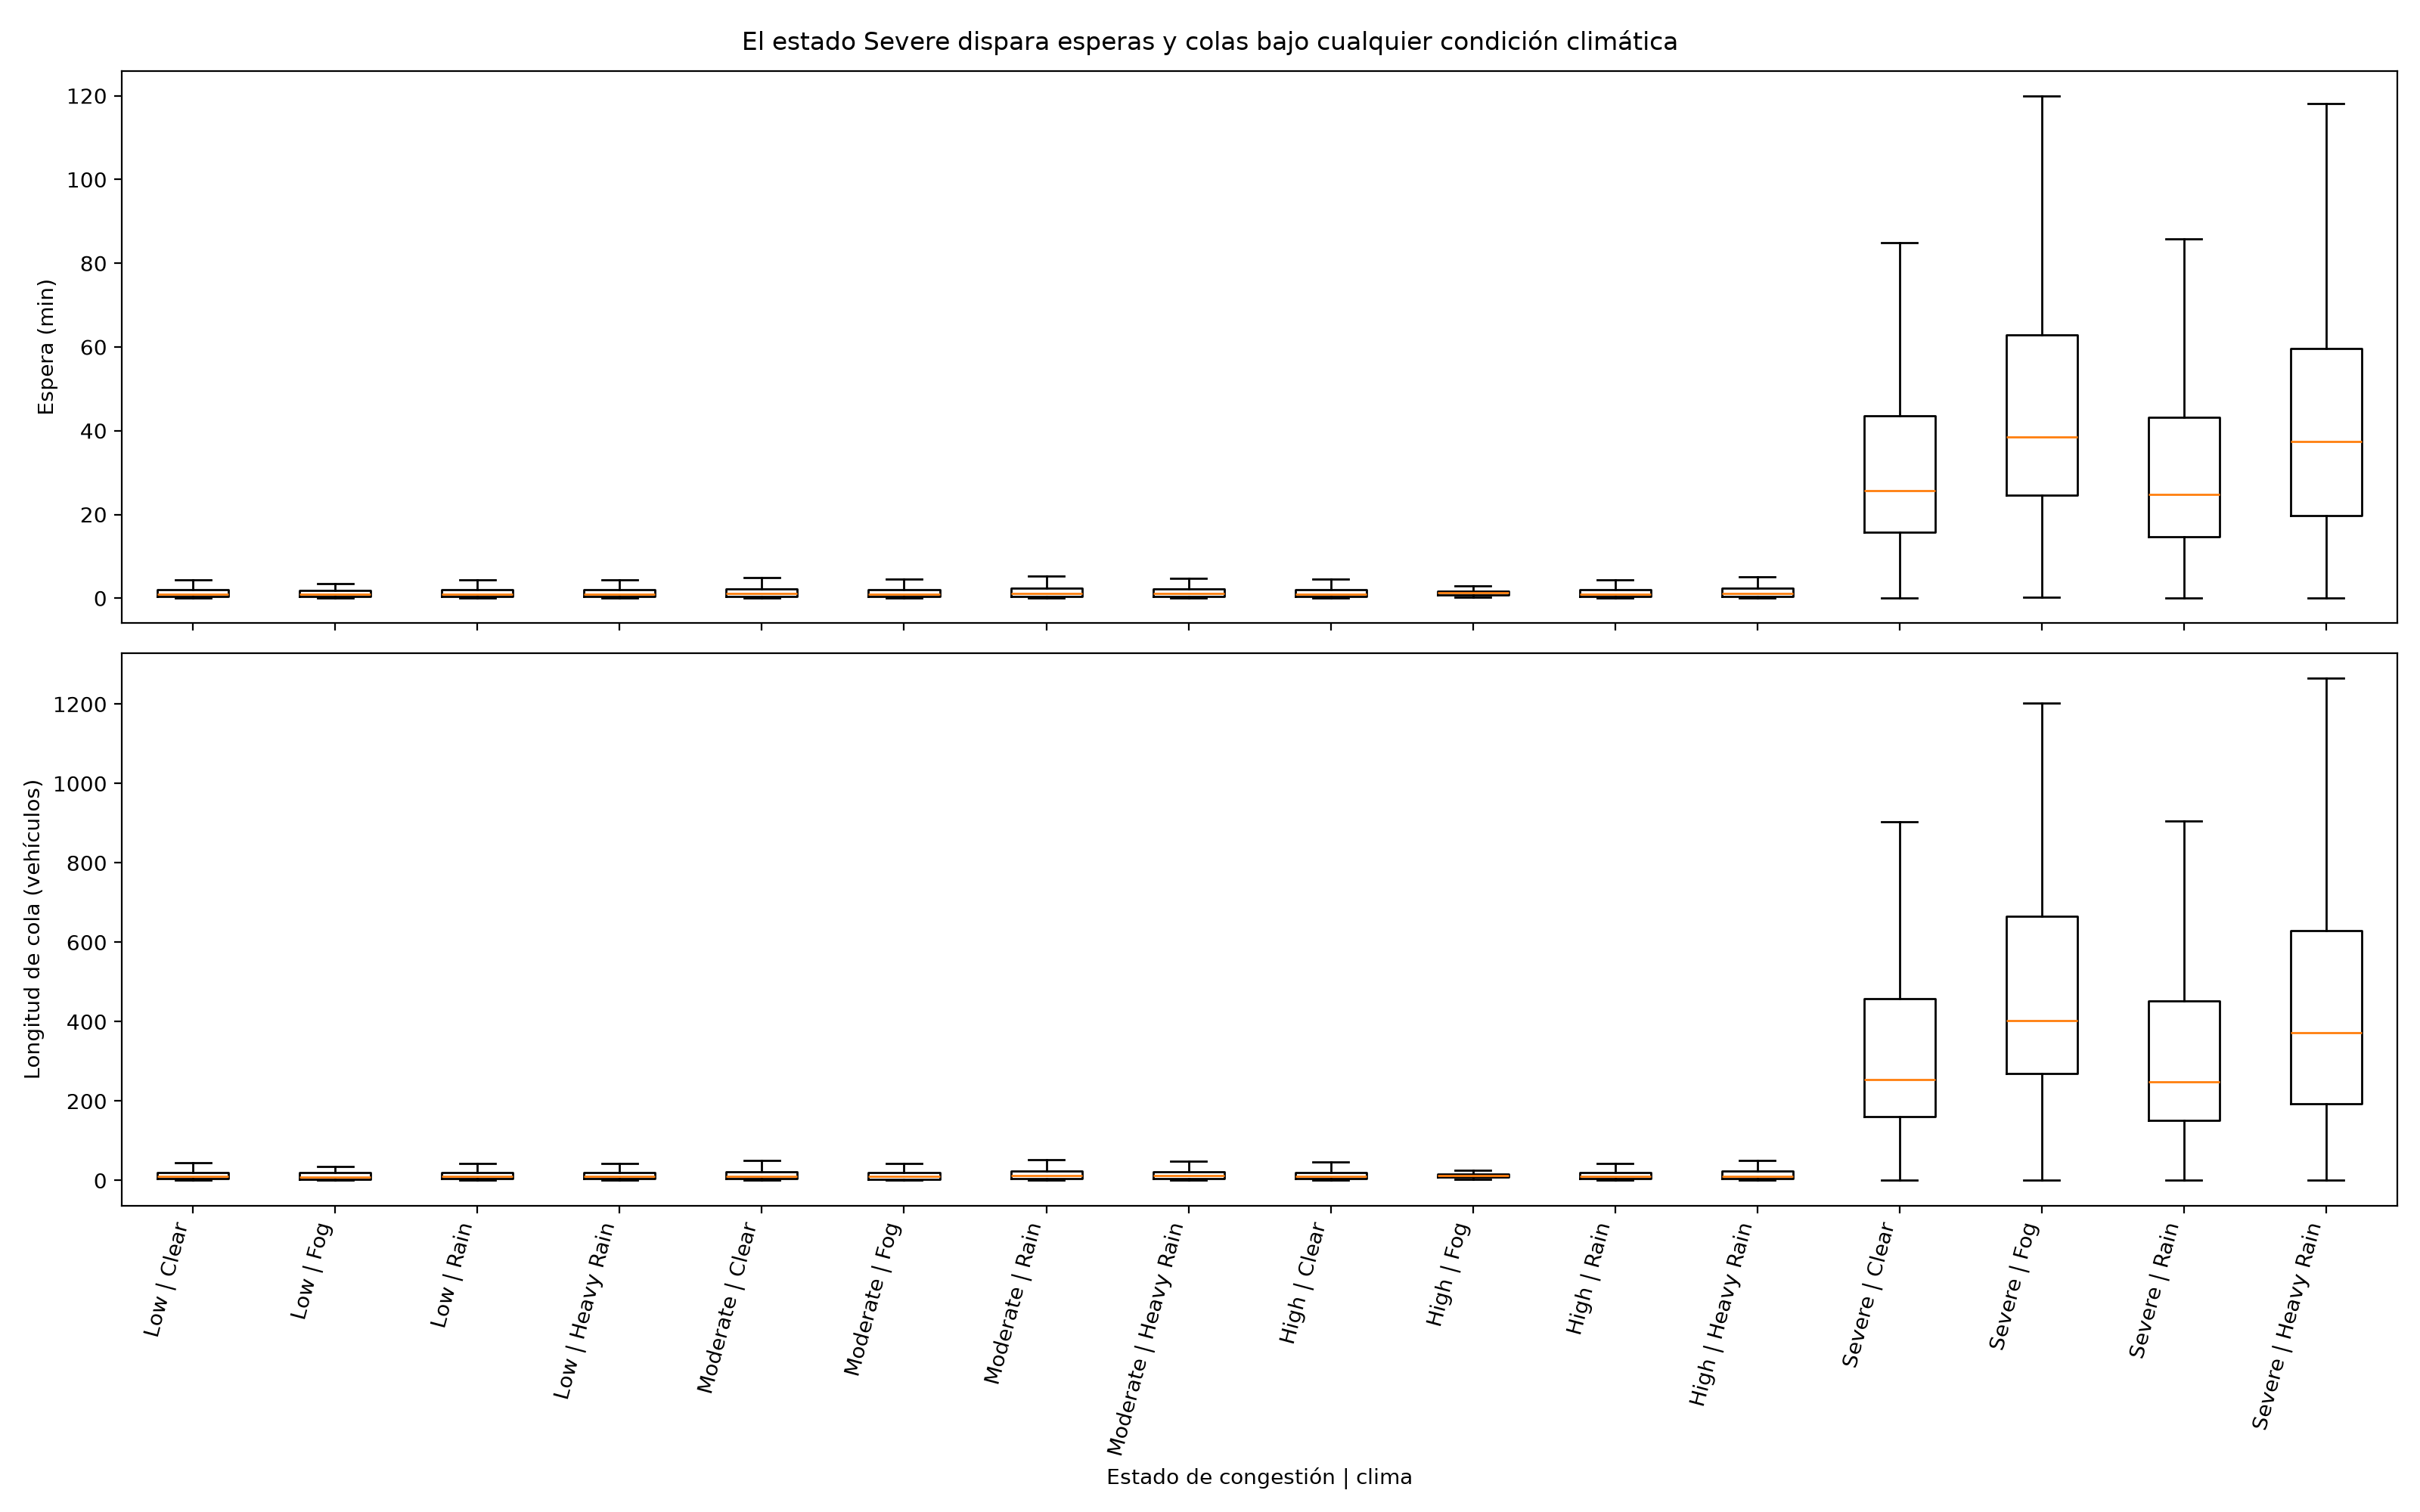
\includegraphics[width=\columnwidth]{boxplot_espera_por_estado_clima.png}
\caption{Distribuciones de espera y longitud de cola por estado y clima.}
\label{fig:box}
\end{figure}

\begin{table}[H]
\caption{Resumen de regímenes y variables operacionales.}
\label{tab:regimes}
\centering\scriptsize
\begin{tabular}{lrrr}
\toprule
Estado--franja & Obs. & $\overline{W}$ (min) & $\overline{Q}$ (veh.)\\
\midrule
Low--Night&66408&1.492&14.924\\
Low--Evening Peak&9671&1.355&13.482\\
Moderate--Night&1586&1.986&19.759\\
Moderate--Evening Peak&10900&1.607&16.111\\
High--Night&5&35.400&361.860\\
High--Evening Peak&6187&1.522&15.285\\
Severe--Night&1&63.800&591.300\\
Severe--Evening Peak&7242&29.221&292.230\\
\bottomrule
\end{tabular}
\end{table}

La categoría Severe presenta una muestra particularmente pequeña en Night: una sola
observación con espera media de 63.800 minutos y cola media de 591.300 vehículos.
Este registro no permite estimar una persistencia estable para ese régimen; se conserva
en el resumen, pero no sustenta una recomendación operativa específica.

La Tabla~\ref{tab:regimes} identifica los principales cortes de lectura del resumen operativo conservado en \texttt{resultados/tablas/tabla\_1\_resumen\_regimenes.csv}; el Cuadro~\ref{tab:tests} presenta las pruebas de homogeneidad y el Cuadro~\ref{tab:queue} resume el ajuste de colas. La simulación SimPy entregó esperas medias de 0.315, 0.506, 0.958, 2.281 y 3.766 minutos para $\rho=0.2,0.4,0.6,0.8,0.9$, respectivamente. El aumento monótono concuerda con la dirección esperada por el modelo, pero usa parámetros sintéticos.

\section{Discusión, limitaciones y conclusiones}
Los contrastes estadísticos y las diferencias entre matrices apoyan la parte no homogénea de la hipótesis para este dataset: permiten rechazar la equivalencia empírica de los regímenes observados. La comparación Night--Clear versus Evening Peak--Rain muestra cambios en las rutas de salida desde estados bajos, moderados y severos; las figuras deben interpretarse junto con los tamaños de muestra y las filas sin transiciones observadas. El ajuste de colas mejora marginalmente al incorporar curvatura, mientras que SimPy confirma una respuesta creciente bajo un servidor semaforizado idealizado.
Las pruebas realizadas no verifican directamente la propiedad de Markov respecto del
historial completo; por tanto, el término CMTD describe una dinámica Markoviana asumida
con transiciones estimadas condicionalmente, no una validación independiente de esa propiedad.

El archivo no contiene aforos de llegada independientes, capacidad calibrada por aproximación ni mediciones de campo para validar $\mu_{\mathrm{ef}}$. La capacidad usada combina carriles, velocidad límite y fracción verde; por ello $\rho$ es un indicador operacional reproducible, no una medición normativa de saturación. Además, los deciles empíricos alcanzan una utilización máxima media de 0.3906 y un máximo observado de 0.6759; la curvatura hacia $\rho\to1$ incorpora por ello una extrapolación funcional reforzada por SimPy, no una observación directa de saturación cercana. La prueba $\chi^2$ detecta diferencias de frecuencias, pero no identifica causalidad entre clima, horario y congestión. Finalmente, el dataset representa los pares disponibles y no garantiza generalización a otras ciudades.

En operación, los resultados justifican separar matrices de transición por horario, clima y tipo de día al monitorear intersecciones, sujetando cada regla a umbrales y aforos locales. La gestión puede priorizar estados High y Severe y revisar planes de verde en regímenes con mayor persistencia observada, sin interpretar este análisis como una demostración de causalidad ni como una calibración automática de semáforos. En conclusión, la evidencia soporta diferencias no homogéneas entre regímenes y un crecimiento creciente de la espera dentro del rango estudiado, con suficiente consistencia para orientar diagnóstico y futuras mediciones, pero no para afirmar transferencia ni causalidad sin aforos de campo.

\bibliographystyle{IEEEtran}
\bibliography{referencias}

\appendices
\section{Herramientas, modelos, skills y trazabilidad}
El flujo fue ejecutado con GitHub Copilot en modo agente dentro de VS Code utilizando
\textbf{Copilot Fusion (\texttt{gpt-5.6-luna})}, el enrutador/combinador automático de modelos de Copilot.
Se preservaron \texttt{AGENTS.md}, el CSV original y las skills propias. Los scripts utilizados
fueron \texttt{01\_preparar\_datos.py}, \texttt{02\_analisis\_markov\_colas.py},
\texttt{03\_validacion\_simpy.py}, \texttt{04\_generar\_diagramas.py},
\texttt{dibujar-grafo.py}, \texttt{recalcular\_valores.py} y
\texttt{revisar\_fuentes.py}. La skill propia \texttt{dibujar-grafo} generó los grafos
dirigidos; \texttt{revisar-fuentes} auditó afirmaciones; \texttt{simpy-discrete-event-simulation}
guió la simulación con procesos, \texttt{Resource} y semillas; y \texttt{paper-writing} guió
estructura, estilo IEEE, figuras, tablas y referencias. La plantilla usa
\texttt{IEEEtran} en modo \texttt{conference}; el pie de página identifica la elaboración
asistida en todas las páginas.

\end{document}
